\documentclass[a4paper,12pt]{article}

\usepackage{rotating}
\usepackage[top=1in, bottom=1in, left=0.75in, right=0.75in]{geometry}
\usepackage{graphicx}
\usepackage[numbers,square,sort&compress]{natbib}
\usepackage{setspace}
\usepackage[cdot,mediumqspace,]{SIunits}
\usepackage{caption}
\usepackage{subcaption}
\usepackage{mathtools}
\usepackage{authblk}
\usepackage{float}
\renewcommand{\thesubsection}{\thesection.\alph{subsection}}
\providecommand{\e}[1]{\ensuremath{\times 10^{#1}}}

\begin{document}
\onehalfspacing
\title{PHY 407 Lab 3}
\author{Natalie Price-Jones, 999091021}
\date{26 September 2014}
\affil{\small{natalie.price.jones@mail.utoronto.ca}}
\maketitle

\section{Question 1}

The following equation was implementated in lab3\_q1.py to calculate the heat capacity as a function of temperature shown in Figure \ref{fig:q1}.

\begin{equation}
C_V = 9V\rho k_B\left(\frac{T}{\theta_D}\right)^3\int_0^{\theta_D/T}\frac{x^4e^x}{(e^x - 1)^2}dx
\label{eqn:Cv}
\end{equation}

\subsection{Part b)}

\begin{figure}[H]
\centering
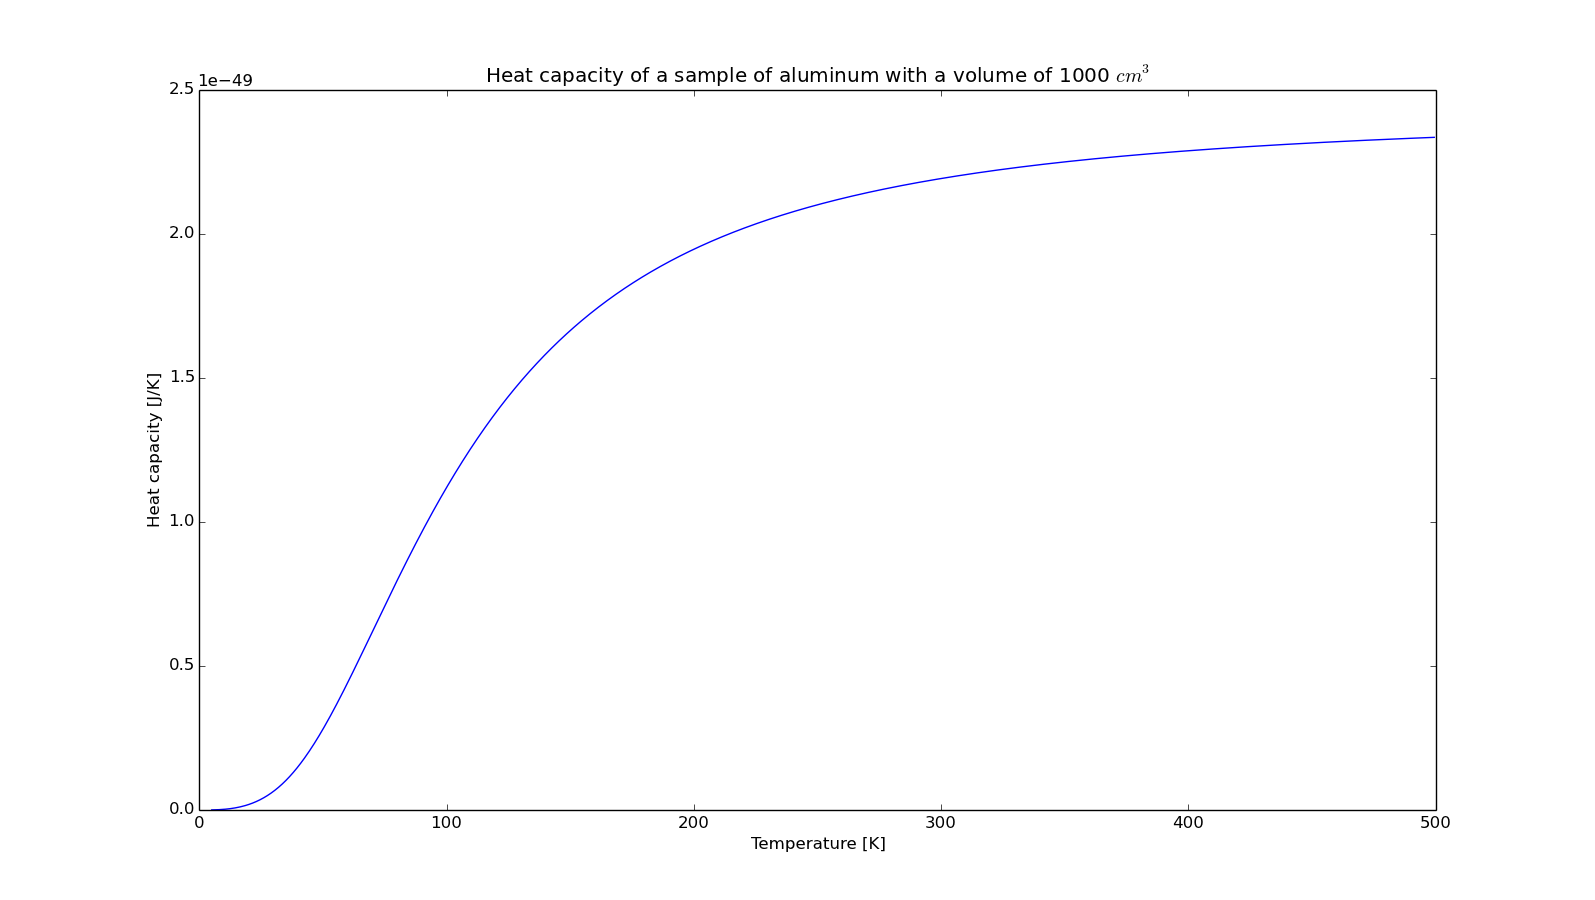
\includegraphics[width = \linewidth]{lab3q1.png}
\caption{Heat capacity of a block of aluminum with a volume of $ V = 1000\,cm^3$, an number density of $\rho = 6.022\e{28}\, m^{-3}$ and a Debye temperature of $\theta_D = 428\,K$.}
\label{fig:q1}
\end{figure}

\section{Question 2}
\subsection{Part b)}

This was a relatively simple function to program (as demonstrated by the brevity of lab3\_q2.py), but required some modification first. 

The original integral is shown below:

\begin{equation}
I = \int_0^{\infty}\frac{z^3}{e^z - 1}dz\nonumber
\end{equation}

Since this integral has one bound at infinity, the first step was to make a change of variables ($z = x/(1-x),\, dz = dx/(1-x)^2$) to make finite bounds. The integral was now:

\begin{equation}
I = \int_0^1\frac{x^3}{(1-x)^5 (e^{x/(1-x)}-1)}dx
\label{eqn:q2int}
\end{equation}

The next step was to decide how to evaluate this integral. The integrand is clearly a well behaved function (Figure \ref{fig:q2meta}), so Gaussian quadrature would be the most accurate method. 

\begin{figure}[H]
\centering
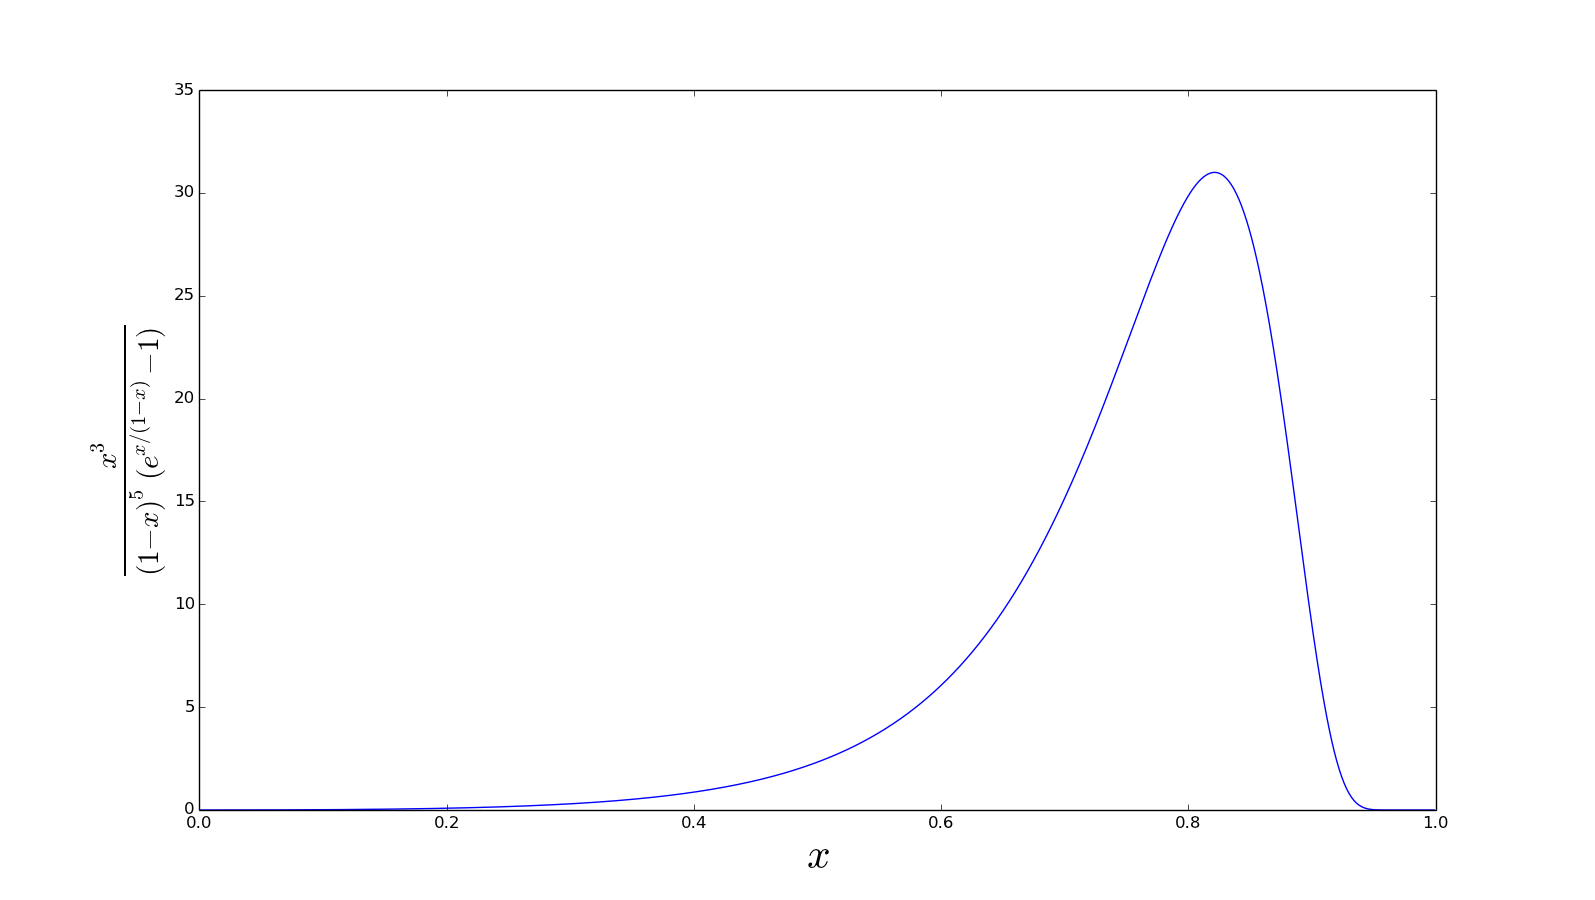
\includegraphics[width = \linewidth]{lab3q2meta.png}
\caption{Behaviour of the integrand of Equation \ref{eqn:q2int} between the bounds of the integral.}
\label{fig:q2meta}
\end{figure}

The result of evaluating the integral was: 6.494.

\subsection{Part c)}

From the result of part b), it was possible to calculate the Stefan-Boltzmann constant ($\sigma$).

\begin{eqnarray}
W &=& \sigma T^4\nonumber\\
W &=& \frac{k_B^4 T^4}{4\pi^2c^2\hbar^3}\int_0^{\infty}\frac{z^3}{e^z - 1}dz\nonumber\\
\implies \sigma &=& \frac{k_B^4}{4\pi^2c^2\hbar^3}\int_0^{\infty}\frac{z^3}{e^z - 1}dz
\label{eqn:sbconst}
\end{eqnarray}

Using Equation \ref{eqn:sbconst} for the Stefan-Boltzmann constant and making the usual change of variables to transform the integral to Equation \ref{eqn:q2int}, it was a simple matter to compute $\sigma = 5.66\e{-8}$. This deviates very little from the known value, $\sigma = 5.67\e{-8}$.

\section{Question 3}
\subsection{Part c)}

It is easy to see in Figure \ref{fig:q3} that the minimum in the forward difference method error corresponds roughly with $h = 10^{-8}$ (marked with a blue dashed line on the plot). This matches with what was expected when considering Equation \ref{eqn:ferr}. Since $C\sim10^{-16}$ for Python, the rounding error dominates below $h\sim 10^{-8}$, while truncation error dominates above this $h$ value. When trucation error dominates, $\epsilon_f \propto h$, so as $h$ increases, $\epsilon_f$ increases. When rounding error dominates, $\epsilon_f \propto h^{-1}$, so as $h$ increases, $\epsilon_f$ decreases. These two regimes are clearly visible in Figure \ref{fig:q3}.

\subsection{Part d)} 

\begin{figure}[H]
\centering
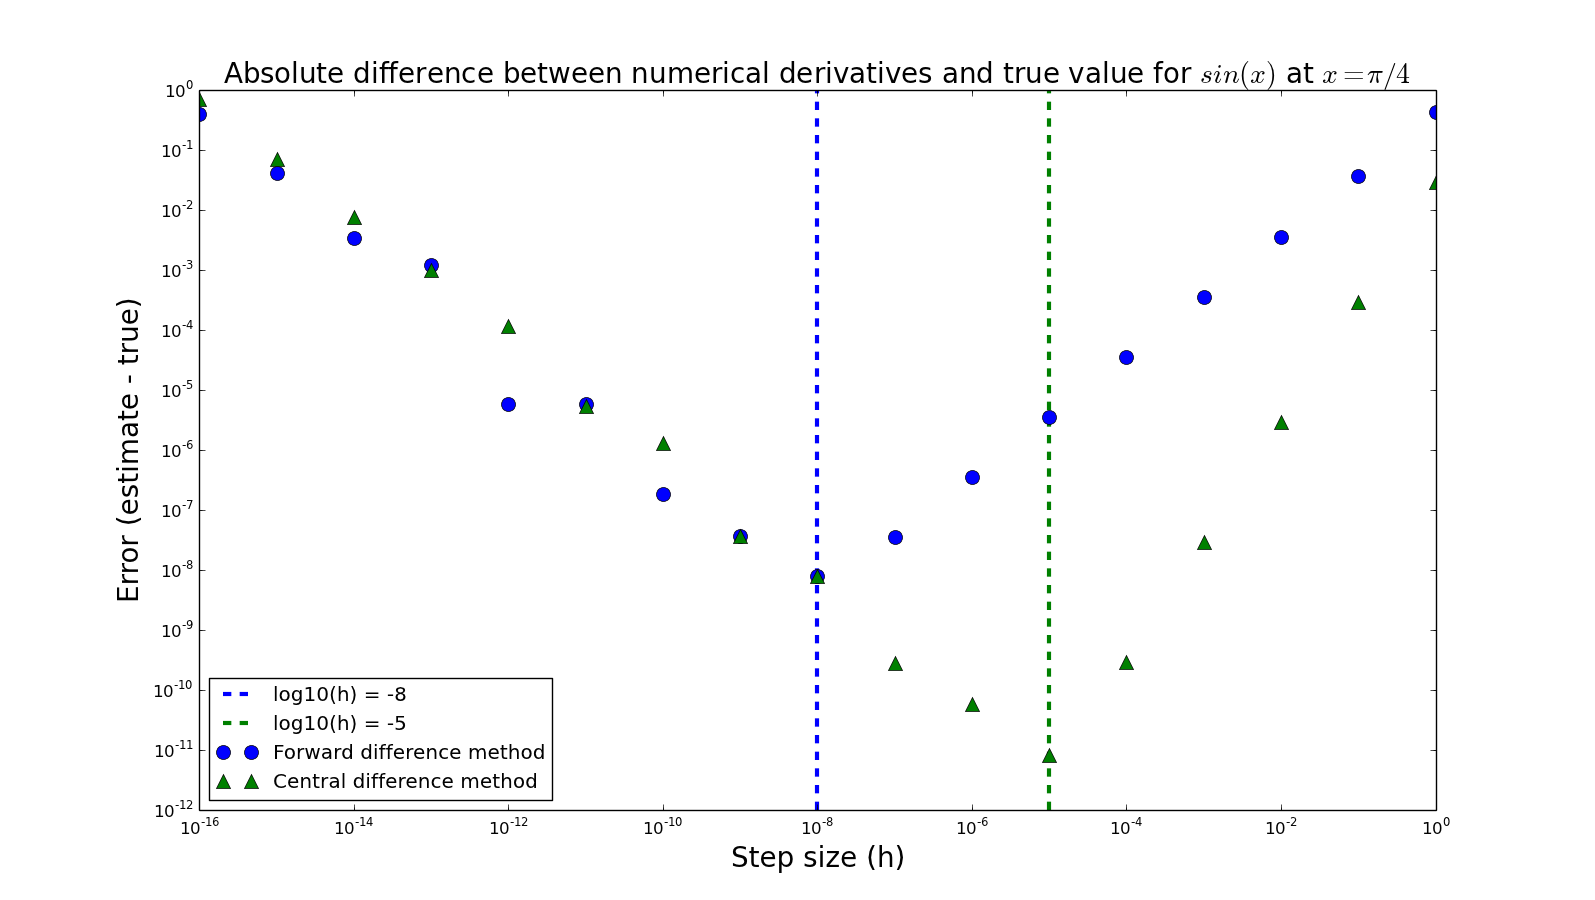
\includegraphics[width = \linewidth]{lab3q3.png}
\caption{Absolute difference between numerical estimation of derivative of $sin(x)$ at $x=\pi/4$ and its true value, $cos(\pi/4) = 1/\sqrt{2}$. Dashed lines (roughly) mark expected minima for the method of the corresponding colour.}
\label{fig:q3}
\end{figure}

It is easy to see from this figure that for $h >\,\sim 10^{-8}$, the central difference method provides results far closer to the true result than the forward difference method. However, for $h \leq\, \sim 10^{-8}$, the central difference and forward difference methods are approximately equally bad. To see why, simply look at the equations that estimate the error in each method.

\begin{eqnarray}
\label{eqn:ferr}
\epsilon_f &=& \frac{2C|f(x)|}{h} + \frac{1}{2}h|f''(x)|\\
\epsilon_c &=& \frac{2C|f(x)|}{h} + \frac{1}{24}h^2|f'''(x)|
\label{eqn:cerr}
\end{eqnarray}

The error in the forward difference method ($\epsilon_f$) is given by Equation \ref{eqn:ferr}, while the error in the central difference method ($\epsilon_c$) is given by Equation \ref{eqn:cerr}, where $C\sim10^{-16}$ for Python.

Both Equation \ref{eqn:ferr} and \ref{eqn:cerr} are composed of two parts. The second term represents the approximation error inherent in the integral, and is different for each method. However the first term is the same for both, and represents the round-off error. As one goes to smaller values for h, the methods become equivalently bad because the round-off error dominates at small h. The fact that the approximation error is generally smaller for the central difference method is eclipsed by the round-off error term, and so it performs only as well as the forward difference method.

\section{Question 4}
\subsection{Part b)}

\begin{figure}[H]
\centering
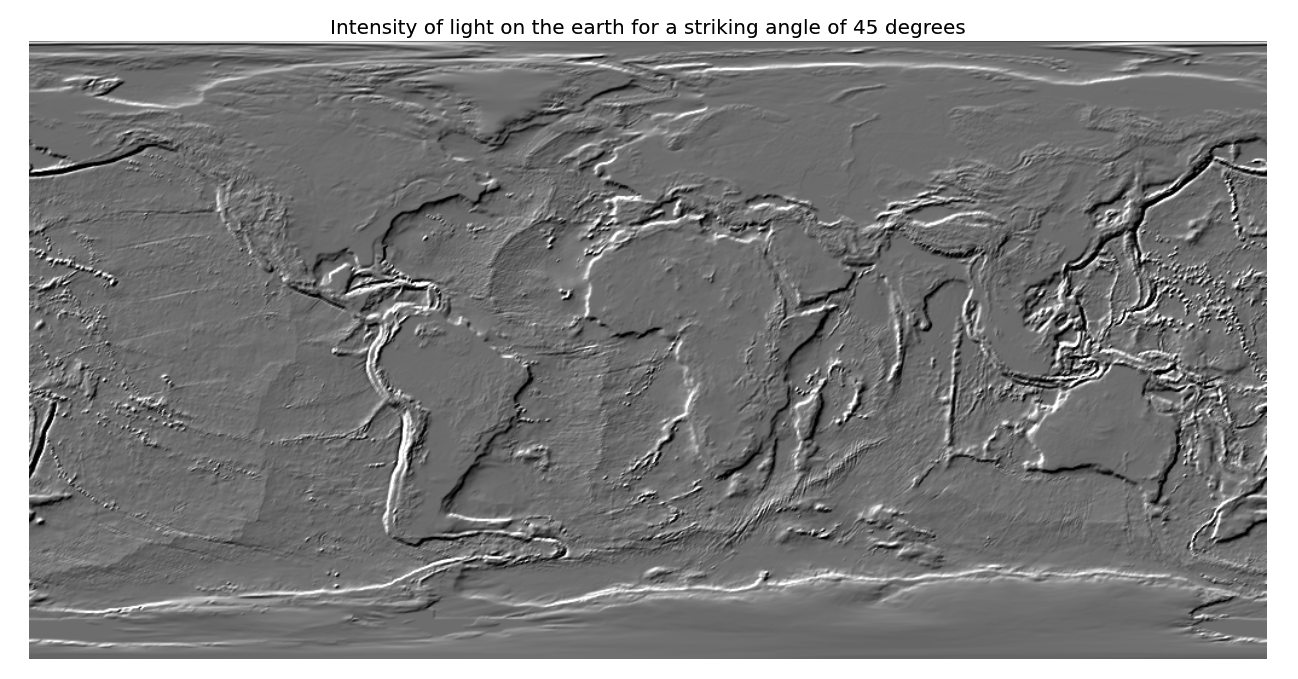
\includegraphics[width = \linewidth]{lab3q4b.png}
\caption{}
\label{fig:q4b}
\end{figure}

\subsection{Part c)}

\begin{figure}[H]
\centering
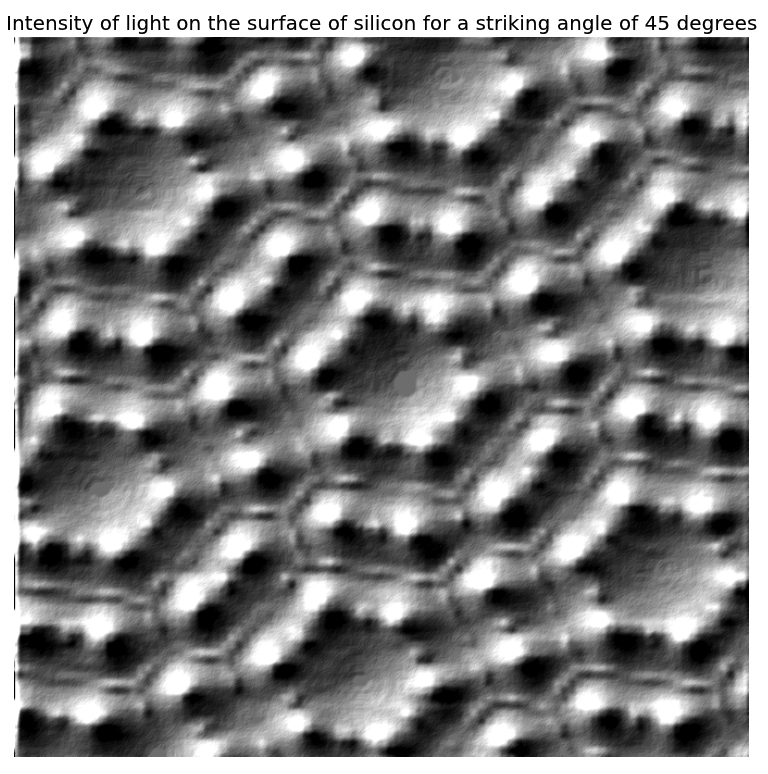
\includegraphics[width = \linewidth]{lab3q4c.png}
\caption{}
\label{fig:q4c}
\end{figure}

\end{document}